\documentclass[twoside, 10pt]{article}

% Русский перевод статьи noether_casimir_drive.tex (рабочий вариант для осмысления).
% Оригинал для подачи — noether_casimir_drive.tex (английский).

\usepackage[T1, T2A]{fontenc}   % Standard package for selecting font encodings
\usepackage[utf8]{inputenc} % Accept different input encodings
\usepackage[english, ukrainian, russian]{babel}

\usepackage{mathptmx}

\usepackage{indentfirst}    % Indent first paragraph after section header

\usepackage{sectsty}        % Control sectional headers

\sectionfont{\normalfont\Large\textbf}
\subsectionfont{\normalfont\large\textbf}

\usepackage{multicol}       % Intermix single and multiple columns
\usepackage{orcidlink}      % Insert hyperlinked ORCiD logo
\usepackage{fancyhdr}       % Extensive control of page headers and footers

\usepackage{filecontents}
\usepackage{hyperref, doi}
\usepackage[numbers]{natbib}

\bibliographystyle{myunsrtnat}

% --- METADATA ---
\def\myfirstpage{1}
\def\mylastpage{15}
\def\mypages{\myfirstpage-\mylastpage}
\def\myfilename{noether_casimir_drive_ru}
\def\myname{А. Дроздов}
\def\mynameukr{А. Дроздов}
\def\mytitle{Теорема Нётер и сотовый двигатель Казимира: о несохранении импульса в асимметричных вакуумных системах}
\def\mytitleukr{Теорема Нетер та стільниковий рушій Казимира: про незбереження імпульсу в асиметричних вакуумних системах}
\def\myissn{2222-5617}
\def\mydoi{10.26565/2222-5617-2026-XX-XX} % ← placeholder, замените при подаче
\def\myemail{alexey.drozdov.07@gmail.com}
\def\ukrvisnyk{Вісник Харківського національного університету імені В.~Н.~Каразіна, серія «Фізика», вип. XX, \mypages~(2026)}
\def\ruvisnyk{Вестник Харьковского национального университета имени В.~Н.~Каразина, серия «Физика», вып. XX, \mypages~(2026)}
\def\myworkplace{Харьковский национальный университет имени В.~Н.~Каразина, пл. Свободы, 4, 61022 Харьков, Украина}
\def\myworkplaceukr{Харківський національний університет імені В.~Н.~Каразіна, майдан Свободи, 4, 61022 Харків, Україна}
\def\myorcidlink{0009-0004-1386-4534}

\def\myreceived{Поступила в редакцию 9 января 2026 г.}
\def\myaccepted{Принята к печати 9 января 2026 г.}
\def\myreceivedukr{Надійшла до редакції 9 січня 2026 р.}
\def\myacceptedukr{Прийнято до друку 9 січня 2026 р.}

\def\licenseref{http://creativecommons.org/licenses/by/4.0/}

\def\myvspacebeforesubsection{-2.0mm}
\def\myvspaceaftersubsection{-2.5mm}

\def\collontitulasfontcode{lmss}

\newcommand{\MyTitle}{\expandafter\MakeUppercase\expandafter{\mytitle}}
\newcommand{\MyTitleUkr}{\expandafter\MakeUppercase\expandafter{\mytitleukr}}

\fancypagestyle{firstpagestyle}{
\renewcommand{\headrulewidth}{0.6pt}
\fancyhead[C]{\ukrvisnyk \\ \ruvisnyk}
\renewcommand{\footrulewidth}{0.6pt}
\fancyfoot[L]{${}^{\copyright}$ \myname}
\fancyfoot[R]{~ \\ \fontencoding{T1}\fontfamily{\collontitulasfontcode}{\selectfont \textit{Open Access. This article is licensed under a Creative Commons Attribution 4.0}} \\
\href{\licenseref}{\fontencoding{T1}\fontfamily{\collontitulasfontcode}{\selectfont \textit{\licenseref}}}}
}

\usepackage{graphicx}
\usepackage{caption}
\DeclareCaptionFormat{nocaption}{}
\captionsetup{format=nocaption,aboveskip=0pt,belowskip=0pt}
\usepackage{float}
\floatplacement{figure}{H}
\usepackage{xcolor}
\usepackage{enumerate}
\usepackage{geometry}
\usepackage{amsmath, amssymb}
\usepackage{textcomp}
\usepackage{upquote}
\usepackage{ucs}
\usepackage{grffile}
\usepackage[Export]{adjustbox}
\adjustboxset{max size={0.9\linewidth}{0.9\paperheight}}
\usepackage{longtable, booktabs, enumitem, ulem, wrapfig, sidecap}

\providecommand{\keywords}[1]{\textbf{\textit{Ключевые слова:}} #1}
\providecommand{\keywordsukr}[1]{\textbf{Ключові слова:} #1}

\author{\myname \,\orcidlink{\myorcidlink}}
\title{\textbf{\MyTitle.}}
\date{}

\definecolor{urlcolor}{rgb}{0,.145,.698}
\definecolor{linkcolor}{rgb}{0,0,0}
\definecolor{citecolor}{rgb}{0,0,0}

\providecommand{\doi}[1]{DOI: \href{https://doi.org/#1}{#1}}

\geometry{verbose,includehead,
nomarginpar,
tmargin=1.1cm,bmargin=3.0cm,lmargin=1.85cm,rmargin=1.85cm}

\setlength{\columnsep}{0.5cm}

% forbid word transfer
\hyphenpenalty=10000

\begin{document}

\fontencoding{T2A}\fontfamily{ptm}\selectfont

\setcounter{page}{\myfirstpage}

\pagestyle{fancy}
\fancyhead{}
\fancyhead[CE]{\fontencoding{T2A}\fontfamily{ptm}{\selectfont \textit{\mytitle.}}}
\fancyhead[CO]{\fontencoding{T2A}\fontfamily{ptm}{\selectfont \textit{\myname}}}
\renewcommand{\headrulewidth}{0.6pt}
\fancyfoot{}
\fancyfoot[LE,RO]{\thepage}
\fancyfoot[LO,RE]{{~} \\ {\fontencoding{T2A}\fontfamily{ptm}{\selectfont \ruvisnyk}} \\ {\fontencoding{T2A}\fontfamily{\collontitulasfontcode}{\selectfont \ukrvisnyk}}}
\fancyfoot[CO,CE]{}

$\,$

\thispagestyle{firstpagestyle}

\vspace{-9.4mm}

\begin{tabular}{lcr}
\doi{\mydoi}
& \,\,\,\,\,\,\,\,\,\,\,\,\,\, \,\,\,\,\,\,\,\,\,\,\,\,\,\, \,\,\,\,\,\,\,\,\,\,\,\,\,\, \,\,\,\,\,\,\,\,\,\,\,\,\,\, \,\,\,\,\,\,\,\,\,\,\,\,\,\, \,\,\,\,\,\,\,\,\,\,\,\,\,\,
& ISSN \myissn (Print)
\end{tabular}

\vspace{9mm}

\begin{tabular}{l}
Оригинальная статья \\
Статья в печати \\
\href{https://doi.org/\mydoi}{https://doi.org/\mydoi} \\
УДК 53.09, 621.3, 629.7 \\
PACS: 11.10.Ef, 03.70.+k, 42.50.Lc \\
\end{tabular}

\section*{\centering {\fontencoding{T2A}\fontfamily{ptm}{\selectfont \MyTitle}}}

\vspace{7mm}
\centerline{\Large{\myname \,\orcidlink{\myorcidlink} }}
\vspace{7.5mm}
\centerline{\textit{\myworkplace}}
\centerline{\textit{E-mail: \href{mailto:\myemail}{\myemail}}}

\vspace{5mm}
\centerline{\myreceived}
\centerline{\myaccepted}

\vspace{5mm}

В работе сотовый двигатель Казимира анализируется с помощью теоремы Нётер.
Рассматриваемая система — идеально проводящая пластина с наноразмерной сотовой структурой
на одной стороне — не обладает трансляционной симметрией вдоль оси, нормальной к пластине,
из-за геометрической асимметрии вакуумных мод по её сторонам.
Вследствие этого вакуумный гамильтониан явно зависит
от координаты \(l\) (эффективной длины резонатора), и по теореме Нётер
соответствующая компонента импульса не сохраняется.
Это несохранение проявляется как результирующая сила квантового вакуума (тяга Казимира).
Показано, что полученное выражение для силы на единицу площади непосредственно отражает это нарушение симметрии
и согласуется как с гамильтоновым подходом, так и с разностью плотностей энергии.
Результат подчёркивает глубокий физический принцип: макроскопическая тяга от квантовых флуктуаций вакуума
возникает потому, что система не инвариантна относительно пространственных трансляций.

\vspace{5mm}

\noindent
\begin{keywords}
\textit{теорема Нётер, эффект Казимира, квантовый вакуум, несохранение импульса, наносоты, тяга Казимира}
\end{keywords}

\vspace{5mm}

\noindent
\textbf{Як цитувати}: \textit{\mynameukr}. \textit{\mytitleukr}. {\ukrvisnyk}. \href{https://doi.org/\mydoi} {https://doi.org/\mydoi}.

\vspace{5mm}

\noindent
\textbf{Как цитировать}: \textit{\myname}. \textit{\mytitle}. {\ruvisnyk}. \href{https://doi.org/\mydoi} {https://doi.org/\mydoi}.

\vspace{5mm}

\newpage

\begin{multicols}{2}

\vspace{\myvspacebeforesubsection}
\subsection*{\centering{\fontencoding{T2A}\fontfamily{ptm}{\selectfont ВВЕДЕНИЕ}}}
\vspace{\myvspaceaftersubsection}

Теорема Нётер устанавливает глубокое соответствие между непрерывными симметриями физической
системы и сохраняющимися величинами. В частности, инвариантность относительно пространственных трансляций влечёт сохранение импульса.
В классической конфигурации Казимира с двумя пластинами система остаётся симметричной относительно трансляций вдоль плоскости пластин,
поэтому поперечный импульс сохраняется; граничные условия влияют только на нормальную компоненту.

Напротив, \textit{однотельный} сотовый двигатель Казимира явно нарушает трансляционную симметрию вдоль оси \(z\)
из-за различных граничных условий на разных сторонах одной пластины: одна сторона гладкая,
а другая покрыта проводящими нанорезонаторами. Эта асимметрия делает вакуумный гамильтониан
\(\langle 0|\hat{\mathcal{H}}|0\rangle\) функцией геометрического параметра \(l\) — эффективной
длины нанорезонаторов.

\vspace{\myvspacebeforesubsection}
\subsection*{\centering{\fontencoding{T2A}\fontfamily{ptm}{\selectfont ТЕОРЕМА НЁТЕР И НЕСОХРАНЕНИЕ ИМПУЛЬСА}}}
\vspace{\myvspaceaftersubsection}

Рассмотрим вакуумный гамильтониан на единицу площади, полученный для сотовой системы:

\begin{figure}
\begin{center}
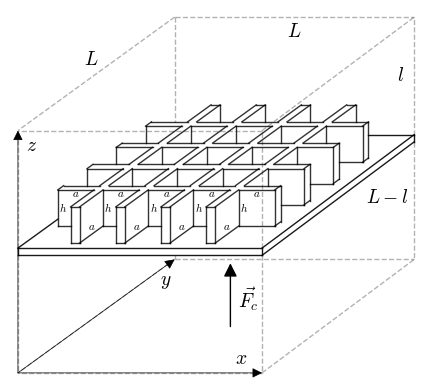
\includegraphics[width=0.42\textwidth]{honeycomb_box_H.png}
\caption{}{\centering{\textbf{Рис.1.} Кубический резонатор с пластиной, покрытой сотами.}}
\end{center}
\label{fig:honeycomb_box_H}
\end{figure}

\end{multicols}

\[
\frac{\langle 0|\hat{\mathcal{H}}|0\rangle}{S} = \frac{\hbar c}{a^2\pi} \Bigg\{
l \sum_{n_x=(0)1}^{\infty}\sum_{n_y=(0)1}^{\infty}
\int_0^{\infty} \sqrt{ \frac{\pi^2}{a^2}(n_x^2 + n_y^2) + k_z^2 } \, dk_z
+ (L - l) \int_0^{\infty}\!\!\int_0^{\infty}
\int_0^{\infty} \sqrt{k_x^2 + k_y^2 + k_z^2} \, dk_z \, \frac{a}{\pi}dk_x \frac{a}{\pi}dk_y
\Bigg\}.
\]

\begin{multicols}{2}

Это выражение явно зависит от \(l\). Следовательно, система \textbf{не инвариантна} относительно бесконечно малых трансляций \(z \to z + \delta z\).

Согласно теореме Нётер, генератор пространственных трансляций — компонента импульса \(P_z\) — сохраняется
\textbf{тогда и только тогда}, когда гамильтониан не зависит от \(z\).
Поскольку \(\partial \langle H \rangle / \partial l \neq 0\), симметрия нарушена,
и \(P_z\) не сохраняется.

Результирующая сила равна
\end{multicols}

\[
\frac{F}{S} = \frac{\partial}{\partial l} \frac{\langle 0|\hat{\mathcal{H}}|0\rangle}{S}
= \frac{\hbar c}{a^2\pi} \left\{
\sum_{n_x=(0)1}^{\infty}\sum_{n_y=(0)1}^{\infty}
\int_0^{\infty} \sqrt{ \frac{\pi^2}{a^2}(n_x^2 + n_y^2) + k_z^2 } \, dk_z
- \int_0^{\infty}\!\!\int_0^{\infty}
\int_0^{\infty} \sqrt{k_x^2 + k_y^2 + k_z^2} \, dk_z \, dn_x dn_y
\right\},
\]

\begin{multicols}{2}
что совпадает с формулой тяги Казимира, полученной ранее через разность плотностей энергии.

Таким образом, появление результирующей тяги не является неожиданным — это следствие нарушенной трансляционной симметрии.
Квантовый вакуум «давит» сильнее с одной стороны, потому что структура мод квантовых вакуумных колебаний различна,
а теорема Нётер даёт фундаментальное объяснение того, почему импульс не обязан сохраняться.



\vspace{\myvspacebeforesubsection}
\subsection*{\centering{\fontencoding{T2A}\fontfamily{ptm}{\selectfont ТЕНЗОР НАТЯЖЕНИЙ ИЗ ПОЛЕЙ МОД РЕЗОНАТОРА: ПОВЕРХНОСТНЫЕ ИНТЕГРАЛЫ И СКАЧОК НА МЕТАЛЛЕ}}}
\vspace{\myvspaceaftersubsection}

В этом разделе тензор натяжений Максвелла вычисляется непосредственно из полей
собственных мод резонатора, без предположения о потоке импульса плоской волны.
Единицы гауссовы, обозначения Тамма.

\textbf{1. Геометрия.} Пластина нулевой толщины лежит в плоскости $z=0$ внутри куба
$L^3$ с идеально проводящими стенками. Со стороны $z>0$ на пластине стоят идеально
проводящие ячейки сечения $a\times a$; их стенки доходят до грани куба $z=l$
(в \cite{Drozdov2024} $l=L/2$). Со стороны $z<0$ находится гладкая сторона пластины и
большая полость $L\times L\times(L-l)$. Каждая полость есть прямоугольный резонатор
$a\times b\times h$: для ячейки $a=b$, $h=l$; для большой полости $a=b=L$, $h=L-l$.
В формулах ниже координата $z$ отсчитывается от той грани резонатора, которая
совпадает с пластиной (для большой полости это $-z$).

\textbf{2. Поля мод.} Обозначим $k_x=\pi n_x/a$, $k_y=\pi n_y/b$, $k_z=\pi n_z/h$,
$K^2=k_x^2+k_y^2$, $k^2=K^2+k_z^2$, $\omega=ck$. Поля TM-моды ($H_z=0$,
$n_x,n_y\ge1$, $n_z\ge0$):
\end{multicols}
\[
\begin{aligned}
E_z&=A\sin k_xx\,\sin k_yy\,\cos k_zz\,\cos\omega t, &
H_z&=0,\\
E_x&=-A\frac{k_xk_z}{K^2}\cos k_xx\,\sin k_yy\,\sin k_zz\,\cos\omega t, &
H_x&=-A\frac{k\,k_y}{K^2}\sin k_xx\,\cos k_yy\,\cos k_zz\,\sin\omega t,\\
E_y&=-A\frac{k_yk_z}{K^2}\sin k_xx\,\cos k_yy\,\sin k_zz\,\cos\omega t, &
H_y&=A\frac{k\,k_x}{K^2}\cos k_xx\,\sin k_yy\,\cos k_zz\,\sin\omega t.
\end{aligned}
\]
Поля TE-моды ($E_z=0$, $n_z\ge1$, $(n_x,n_y)\ne(0,0)$):
\[
\begin{aligned}
H_z&=A\cos k_xx\,\cos k_yy\,\sin k_zz\,\cos\omega t, &
E_z&=0,\\
H_x&=-A\frac{k_xk_z}{K^2}\sin k_xx\,\cos k_yy\,\cos k_zz\,\cos\omega t, &
E_x&=-A\frac{k\,k_y}{K^2}\cos k_xx\,\sin k_yy\,\sin k_zz\,\sin\omega t,\\
H_y&=-A\frac{k_yk_z}{K^2}\cos k_xx\,\sin k_yy\,\cos k_zz\,\cos\omega t, &
E_y&=A\frac{k\,k_x}{K^2}\sin k_xx\,\cos k_yy\,\sin k_zz\,\sin\omega t.
\end{aligned}
\]
\begin{multicols}{2}

\textbf{3. Проверка полей.} Подстановкой проверяется, что
$\nabla\cdot\mathbf E=\nabla\cdot\mathbf H=0$,
$\nabla\times\mathbf E=-\frac1c\partial_t\mathbf H$,
$\nabla\times\mathbf H=\frac1c\partial_t\mathbf E$ при $\omega=ck$, и что выполнены
граничные условия идеального проводника: касательное $\mathbf E$ и нормальное
$\mathbf H$ обращаются в нуль на всех шести гранях (на $x=0,a$: $E_y=E_z=0$, $H_x=0$;
на $y=0,b$: $E_x=E_z=0$, $H_y=0$; на $z=0,h$: $E_x=E_y=0$, $H_z=0$). Эти соотношения
были дополнительно проверены численно для мод $(2,1,3)$ при $a:b:h=1:1{,}3:2{,}7$
(невязка порядка $10^{-9}$).

\textbf{4. Компонента тензора.} По Тамму
$T_{ik}=\frac1{4\pi}(E_iE_k+H_iH_k)-\frac{\delta_{ik}}{8\pi}(E^2+H^2)$, и сила на тела
внутри замкнутой поверхности равна $\oint T_{ik}n_k\,dS$ (внешняя нормаль). Отсюда
\[
T_{zz}=\frac1{8\pi}\left(E_z^2+H_z^2-E_x^2-E_y^2-H_x^2-H_y^2\right).
\]
Поток импульса $\Pi_{ik}=-T_{ik}$; давление на горизонтальную площадку обозначим
$p\equiv-\langle T_{zz}\rangle$.

\textbf{5. Усреднение по сечению и по периоду.} Усредняем по площади $S=ab$ и по
периоду $2\pi/\omega$. При $n_x,n_y\ge1$ каждый множитель $\sin^2$ или $\cos^2$ по
$x$, по $y$ и по $t$ даёт $\tfrac12$. Для TM-моды:
\end{multicols}
\[
\langle E_z^2\rangle=\frac{A^2}{8}\cos^2k_zz,\qquad
\langle E_x^2+E_y^2\rangle=\frac{A^2}{8}\frac{k_x^2+k_y^2}{K^4}k_z^2\sin^2k_zz=\frac{A^2}{8}\frac{k_z^2}{K^2}\sin^2k_zz,\qquad
\langle H_x^2+H_y^2\rangle=\frac{A^2}{8}\frac{k^2}{K^2}\cos^2k_zz .
\]
\[
8\pi\langle T_{zz}\rangle=\frac{A^2}{8}\left[\cos^2k_zz\left(1-\frac{k^2}{K^2}\right)-\frac{k_z^2}{K^2}\sin^2k_zz\right]
=-\frac{A^2}{8}\frac{k_z^2}{K^2}\left(\cos^2k_zz+\sin^2k_zz\right)=-\frac{A^2}{8}\frac{k_z^2}{K^2},
\]
\begin{multicols}{2}
\noindent где использовано $1-k^2/K^2=-k_z^2/K^2$. Плотность энергии
$w=(E^2+H^2)/8\pi$ той же моды:
$8\pi\langle w\rangle(z)=\frac{A^2}{8}\left[\cos^2k_zz+\frac{k_z^2}{K^2}\sin^2k_zz+\frac{k^2}{K^2}\cos^2k_zz\right]$;
после усреднения ещё и по $z$ (при $n_z\ge1$)
$8\pi\overline w=\frac{A^2}{16}\cdot\frac{K^2+k_z^2+k^2}{K^2}=\frac{A^2}{8}\frac{k^2}{K^2}$.
Следовательно,
\[
p=-\langle T_{zz}\rangle=\overline w\,\frac{k_z^2}{k^2}.
\]
Для TE-моды те же шаги дают
$\langle H_z^2\rangle=\frac{A^2}{8}\sin^2k_zz$,
$\langle H_x^2+H_y^2\rangle=\frac{A^2}{8}\frac{k_z^2}{K^2}\cos^2k_zz$,
$\langle E_x^2+E_y^2\rangle=\frac{A^2}{8}\frac{k^2}{K^2}\sin^2k_zz$, откуда
$8\pi\langle T_{zz}\rangle=-\frac{A^2}{8}\frac{k_z^2}{K^2}$ и тот же результат
$p=\overline w\,k_z^2/k^2$. Если один из поперечных индексов равен нулю (это
возможно только для TE), соответствующий $\cos^2$ равен $1$ вместо $\tfrac12$;
общий множитель удваивается и в давлении, и в энергии, отношение не меняется.
Мода TM с $n_z=0$ имеет $k_z=0$ и давления не создаёт.

\textbf{6. Независимость от $z$.} В п.~5 зависимость от $z$ выпала
($\cos^2+\sin^2=1$). Общая причина: в вакууме
$\partial T_{zk}/\partial x_k=\frac1{4\pi c}\,\partial_t[\mathbf E\times\mathbf H]_z$,
а среднее по периоду от производной по времени равно нулю. При интегрировании
по сечению остаются потоки через боковые стенки:
$T_{zx}=\frac1{4\pi}(E_zE_x+H_zH_x)$, и на стенках $x=0,a$ имеем $E_z=0$
(касательное поле) и $H_x=0$ (нормальное поле), то есть $T_{zx}=0$; то же для
$T_{zy}$ на $y=0,b$. Поэтому
$\frac{d}{dz}\int\langle T_{zz}\rangle\,dx\,dy=0$. Подчеркнём: от $z$ не зависит
только интеграл по сечению; в отдельной точке $(x,y)$ величина $T_{zz}$ меняется
с $z$. В силу входит именно интеграл.

\textbf{7. Нулевые колебания.} Каждая мода есть осциллятор; в основном состоянии
её энергия равна $\hbar\omega/2$, причём электрическая и магнитная части равны
по $\hbar\omega/4$. Это ровно то распределение, которое даёт классическое
усреднение по периоду в п.~5, если амплитуду выбрать так, что
$\overline w\,V=\hbar\omega/2$. Поэтому вклад моды в давление
$p_{\text{моды}}=\frac{\hbar\omega}{2V}\frac{k_z^2}{k^2}$, а давление в полости
\[
p=\frac{\hbar c}{2V}\sum_{\text{моды}}\frac{k_z^2}{k},
\]
где сумма идёт по TM- и TE-модам с указанными в п.~2 областями индексов.
От суммы для энергии, ф.~(1) работы \cite{Drozdov2024}, она отличается только
слагаемым: $k_z^2/k$ вместо $k$.

\textit{Тождество с гамильтоновым подходом.} При $k_z=\pi n_z/h$ имеем
$\partial k/\partial h=-k_z^2/(kh)$, и для каждой моды
\[
-\frac{\partial}{\partial h}\frac{\hbar ck}{2}=\frac{\hbar c}{2h}\frac{k_z^2}{k}=S\,p_{\text{моды}},\qquad V=Sh .
\]
Сила, найденная через тензор натяжений, совпадает с $-\partial E/\partial h$
помодово, до какой-либо регуляризации.

\textbf{8. Поверхности $z=\mathrm{const}$ для сотовой пластины.} Из пп.~5--7:
\begin{itemize}
\item $z\to0^+$ (вакуум у дна ячейки), $z=d$ с $0<d<l$, $z\to l^-$ (у вспомогательной
стенки куба): $-\langle T_{zz}\rangle=p_{\text{cell}}=\frac{\hbar c}{2a^2l}\sum_{\text{ячейка}}\frac{k_z^2}{k}$;
\item $z\to0^-$ (вакуум у гладкой стороны), $z=-d'$ с $0<d'<L-l$, $z\to-(L-l)^+$:
$-\langle T_{zz}\rangle=p_{\text{big}}=\frac{\hbar c}{2L^2(L-l)}\sum_{\text{большая}}\frac{k_z^2}{k}$;
\item внутри металла пластины и стенок: $T_{ik}=0$.
\end{itemize}
Плоскость $z=d$ в области ячеек пересекает их стенки; при нулевой толщине стенок
они в интеграл не дают вклада, и ячейки покрывают всю площадь пластины.

\textbf{9. Скачок на поверхности металла.} На грани $z=0$ (вакуум снаружи, металл
внутри, где поля равны нулю) граничные условия требуют непрерывности
касательного $\mathbf E$ и нормального $\mathbf H$; со стороны вакуума они равны
нулю: $E_x=E_y=0$, $H_z=0$. Нормальное $\mathbf E$ и касательное $\mathbf H$
испытывают скачок на $4\pi\sigma$ и $\frac{4\pi}{c}\mathbf i$ соответственно и со
стороны вакуума отличны от нуля. Поэтому
\[
T_{zz}\big|_{\text{вакуум}}=\frac1{8\pi}\left(E_z^2-H_x^2-H_y^2\right),\qquad
T_{zz}\big|_{\text{металл}}=0 .
\]
Явно, для TM-моды при $z=0$: $\langle E_z^2\rangle=\frac{A^2}{8}$,
$\langle H_x^2+H_y^2\rangle=\frac{A^2}{8}\frac{k^2}{K^2}$, откуда
$-\langle T_{zz}\rangle(0^+)=\frac{A^2}{64\pi}\left(\frac{k^2}{K^2}-1\right)=\frac{A^2}{64\pi}\frac{k_z^2}{K^2}=\overline w\,\frac{k_z^2}{k^2}$,
то есть то же значение, что в объёме полости (п.~6). Для TE-моды при $z=0$
$E_z=0$ и $-\langle T_{zz}\rangle(0^+)=\frac{1}{8\pi}\langle H_x^2+H_y^2\rangle=\overline w\,k_z^2/k^2$.
Скачок $[\![T_{zz}]\!]=T_{zz}|_{\text{металл}}-T_{zz}|_{\text{вакуум}}=p$ есть
поверхностная сила на единицу площади, действующая на поверхностные заряды
$\sigma=E_n/4\pi$ в поле $E_n$ и на поверхностные токи
$\mathbf i=\frac{c}{4\pi}[\mathbf n\times\mathbf H]$ в поле $\mathbf H_t$:
\[
\frac{f_z}{S}=\frac1{8\pi}\left(\langle H_t^2\rangle-\langle E_n^2\rangle\right).
\]
В вакуумном состоянии $\langle\sigma\rangle=0$ и $\langle\mathbf i\rangle=0$, но
корреляции $\langle\sigma E_n\rangle$ и $\langle\mathbf i\times\mathbf H\rangle$ отличны от
нуля: сила квадратична по полям. Для TE-мод на гранях $xy$ поверхностного заряда
нет вовсе ($E_n=E_z=0$), и скачок тензора создают только поверхностные токи; это
явный пример случая, указанного в замечании к \S\,33 Тамма: скачок тензора на
поверхности, не несущей заряда. Для TM-мод флуктуирующие заряды уменьшают давление
на $\langle E_n^2\rangle/8\pi$.

\textbf{10. Сила на пластину.} Возьмём замкнутую поверхность из граней $z=z_1$
($0<z_1\le l$) и $z=-z_2$ ($0<z_2\le L-l$), охватывающих всё сечение $L\times L$;
боковые грани лежат на стенках куба, где $T_{zx}=T_{zy}=0$ (п.~6). Тогда
\[
F_z=\left[\langle T_{zz}\rangle(z_1)-\langle T_{zz}\rangle(-z_2)\right]L^2=(p_{\text{big}}-p_{\text{cell}})\,L^2,
\]
и результат не зависит от $z_1$, $z_2$. При $z_1,z_2\to0$ это сумма двух скачков на
гранях пластины (сила приложена к поверхностям металла); при $z_1=l$,
$z_2=L-l$ это грани у вспомогательных стенок куба (при $l=L/2$ --- грани
$z=\pm L/2$ выше); промежуточные положения дают то же самое. $F_z>0$ (толчок в
сторону ячеек) при $p_{\text{big}}>p_{\text{cell}}$.

\textbf{11. Проверка на двух пластинах Казимира.} Пластины при $z=0$ и $z=a$,
внешние полости до $z=\pm L/2$. В зазоре $k_z=\pi n/a$, поперечный спектр
непрерывен; на единицу площади (две поляризации)
\[
p_{\text{in}}=\frac{\hbar c}{a}\sum_{n\ge1}\int\frac{d^2k_\parallel}{(2\pi)^2}\frac{k_z^2}{k}
\]
(мода $n=0$ имеет $k_z=0$ и не даёт давления), а снаружи сумма по $n$ заменяется
на $\frac a\pi\int dk_z$. По п.~6 значение $p_{\text{in}}$ одно и то же в центре
зазора и у внутренней поверхности каждой пластины, а $p_{\text{out}}$ --- у внешней
поверхности каждой пластины и на гранях $z=\pm L/2$ (при $L\to\infty$ это значение
свободного вакуума). С обрезанием $e^{-k/k_m}$ разность $p_{\text{in}}-p_{\text{out}}$
равна $-0{,}041043$, $-0{,}041110$, $-0{,}041120$ в единицах $\hbar c/a^4$ при
$k_ma=20$, $50$, $100$ и стремится к $-\pi^2/240=-0{,}041123$. Знак означает
притяжение пластин; с плотностью энергии Казимира
$u=-\pi^2\hbar c/720a^4$ это соотношение $p=3u$ \cite{BrownMaclay1969}.

\textbf{12. Ограничения и самокритичные замечания.}

(а) \textit{Приложение B работы \cite{Drozdov2024}.} Там давление на грань $xy$
вычислялось как $\langle H_x^2+H_y^2\rangle/8\pi$. Для электрических (TM) мод
пропущен член $-\langle E_z^2\rangle/8\pi$. С ним отношение давления к плотности
энергии равно $k_z^2/k^2$ для мод обоих типов, а не $1$ для электрической моды
(численно для моды $(2,1,3)$: $0{,}2119$ вместо $1{,}0000$). Поэтому значение $1$ для
электрической моды и опирающееся на него неравенство $F/S\ge\delta(E/V)$ в разделе
«О неполноте стандартного баланса импульса» требуют пересмотра. Гамильтонов вывод
приложения C при этом не затрагивается: по п.~7 он помодово совпадает с тензорным.

(б) \textit{Регуляризация.} С обрезанием $f(k/k_m)$ производная энергии моды равна
$-\partial_h\!\left[\frac{\hbar ck}{2}f\right]=\frac{\hbar c}{2h}\frac{k_z^2}{k}\left[f+\frac{k}{k_m}f'\right]$,
а регуляризованная тензорная сумма $\sum(k_z^2/k)f$ не содержит второго члена.
Для двух пластин различие исчезает при $k_ma\to\infty$ (п.~11). Для сот при конечном
$ak_m$ это не вычислено; возможно, именно этот член связан с зависимостью
$R(ak_m)$. Какая из двух регуляризованных величин физична, в модели идеального
проводника с модовым обрезанием решить нельзя; для этого нужна реальная
$\varepsilon(\omega)$, как в \cite{DLP1961}.

(в) \textit{Высота ячеек.} Расчёт предполагает, что стенки ячеек доходят до грани
куба, и ячейка является замкнутым резонатором. Для реальных ячеек высотой $h\ll L$
ячейка открыта в большую полость, моды не разделяются, и этот расчёт такой случай
не описывает.

(г) \textit{Идеальный проводник.} Скачок есть свойство идеального проводника. В
реальном металле $T_{zz}$ спадает до нуля на толщине скин-слоя, а интеграл силы по
слою равен скачку, пока ток в металле согласован с полем: $\mathbf j=\frac c{4\pi}\nabla\times\mathbf H$.

(д) \textit{Толщина стенок.} Стенки ячеек конечной толщины не несут $z$-силы
($T_{zx}=0$ на них), но уменьшают долю площади пластины, занятую полостями.

(е) \textit{Квантовое среднее.} Равенство электрической и магнитной частей
энергии моды в основном состоянии (п.~7) использовано как стандартный результат
для осциллятора и здесь не выводится.

(ж) \textit{Что проверено.} Численно проверены поля и средние для отдельных мод
и предельное значение для двух пластин. Сумма $\sum k_z^2/k$ для сотовой пластины с
регуляризацией по формуле Эйлера--Маклорена \cite{Drozdov2024} ещё не вычислена.

\vspace{\myvspacebeforesubsection}
\subsection*{\centering{\fontencoding{T2A}\fontfamily{ptm}{\selectfont ТЕНЗОР НАТЯЖЕНИЙ ИЗ СУММЫ НУЛЕВЫХ КОЛЕБАНИЙ}}}
\vspace{\myvspaceaftersubsection}

В работе \cite{Drozdov2024} сила получена из энергии нулевых колебаний
$\frac12\sum\hbar\omega$, вычисленной по двумерной формуле Эйлера--Маклорена;
сам тензор натяжений Максвелла там не выводился. Он следует из той же суммы по модам.

\textbf{Одна мода.} Для плоской волны с волновым вектором $\mathbf{k}$ и плотностью
энергии $u$ поток импульса равен $\Pi_{ij}=u\,k_ik_j/k^2$ (натяжение по Тамму
$T_{ij}=-\Pi_{ij}$). Стоячая волна есть сумма волн с $\pm k_z$ и имеет тот же
$\Pi_{zz}$. Нулевая мода в полости объёма $V$ имеет $u=\hbar\omega/2V$, поэтому
\[
\langle\Pi_{zz}\rangle=\frac{\hbar c}{2V}\sum_{n_x,n_y,n_z}\frac{k_z^2}{k}.
\]
От суммы для энергии, ф.~(1) работы \cite{Drozdov2024},
$E = \frac{1}{2}\sum\,\hbar\omega = \hbar\,c\frac{1}{2}\sum\limits_{n_x}^{}\sum\limits_{n_y}^{}\sum\limits_{n_z}^{}k.$,
это отличается только
слагаемым: $k_z^2/k$ вместо $k$.

\textbf{Связь с гамильтонианом.} При $k_z=\pi n_z/l$ имеем
$\partial k/\partial l=-k_z^2/(k\,l)$, так что для каждой моды в отдельности
\[
-\frac{\partial}{\partial l}\,\frac{\hbar c\,k}{2}=\frac{\hbar c}{2\,l}\,\frac{k_z^2}{k}
= S\,\Pi_{zz}^{\mathrm{(моды)}},\qquad V=S\,l .
\]
Таким образом, $-\partial E/\partial l=S\,\Pi_{zz}$ выполняется помодово (теорема
Гельмана--Фейнмана \cite{Feynman1939}; иначе говоря, сохранение адиабатического
инварианта $E/\omega$ каждой моды при медленном сдвиге стенки). Поэтому
гамильтонова сила $\partial\langle H\rangle/\partial l$ предыдущих разделов и сила,
найденная через тензор натяжений, совпадают ещё до регуляризации.

\textbf{Регуляризация.} Регуляризующая функция $f(k/k_m)$ и процедура
Эйлера--Маклорена из \cite{Drozdov2024} применяются без изменений, только функция
$G$ строится из $k_z^2/k$. При конечном $k_m$ два выражения могут отличаться на
члены с $f'(k/k_m)$, поскольку $f$ зависит от $|\mathbf{k}|$. Являются ли эти члены
источником зависимости от материала $R(ak_m)$, ещё предстоит проверить расчётом.

\textbf{Проверка симметрией.} Перенормированный тензор $\langle T_{\mu\nu}\rangle$
электромагнитного поля бесследов. Между двумя параллельными пластинами граничные
условия инвариантны относительно бустов вдоль пластин; вместе с условием на след это
даёт $\langle\Pi_{zz}\rangle=3\langle u\rangle$ (Браун и Маклей \cite{BrownMaclay1969}),
то есть множитель $F/S=-3\,\delta(E/V)$, найденный в \cite{Drozdov2024} для
конфигурации Казимира. Ячейка сот --- волновод вдоль $z$: вдали от торцов её
граничные условия инвариантны относительно бустов вдоль $z$, поэтому в блоке $(t,z)$
$\langle T_{\mu\nu}\rangle\propto\eta_{\mu\nu}$ и $\langle\Pi_{zz}\rangle=-\langle u\rangle$.
Это воспроизводит $|F/S|=\delta(E/V)$ из приложений~B и~C работы \cite{Drozdov2024}.
Аргумент точен для идеального проводника в пределе $ak_m\to\infty$ и с точностью до
торцевых поправок порядка $a/l$; обрезание материала нарушает буст-инвариантность, и
поправки от него требуют суммы по модам, приведённой выше.

Тот же поток можно вычислить без модового обрезания методом Дзялошинского, Лифшица и
Питаевского \cite{DLP1961}: натяжение в вакуумном зазоре находится из функции Грина
поля, а материал входит через $\varepsilon(\omega)$. Для ячейки сот для этого нужна
функция Грина прямоугольного волновода; это оставлено для дальнейшей работы.

\vspace{\myvspacebeforesubsection}
\subsection*{\centering{\fontencoding{T2A}\fontfamily{ptm}{\selectfont О ВСПОМОГАТЕЛЬНОМ РЕЗОНАТОРЕ И ПОЛОЖЕНИИ ГРАНЕЙ КОРОБОЧКИ}}}
\vspace{\myvspaceaftersubsection}

Идеально проводящие стенки куба $L^3$ (рис.~2), как и у Казимира, --- вспомогательное
граничное условие, не имеющее физического прообраза, подобно периодическим граничным
условиям, которыми в учебниках квантовой механики нормируют плоские волны. Процедура
законна потому, что результат берётся в пределе $L\to\infty$. По теореме Вейля
\cite{Weyl1912} главный член числа мод, $N(k)\simeq Vk^3/3\pi^2$, не зависит от
граничных условий на внешних гранях: от них зависят лишь поверхностные поправки, и
вклад удалённых стенок в силу на пластину исчезает при $L\to\infty$. Конечный ящик
делает дискретными волновые числа, но не пространство. Обрезание $k_m$ --- отдельный,
физический элемент: его задаёт прозрачность материала пластины для коротких волн.
(Если считать вакуум дискретной средой с шагом решётки $b$, её зона Бриллюэна дала бы
ещё обрезание $|\mathbf{k}|\le\pi/b$; однако для силы на пластину существенно обрезание
материала пластины.)

\textbf{Положение граней коробочки.} Поставим грани при $z=\pm d$, $0<d<L/2$, строго
внутри двух полостей. Вещества в полости нет, поэтому $\partial_k\langle T_{zk}\rangle=0$.
После интегрирования по сечению ячейки поток через боковые стенки обращается в нуль:
на идеальном проводнике $E_z=0$ (касательная) и $H_n=0$ (нормальная), так что
$T_{zn}=(E_zE_n+H_zH_n)/4\pi=0$. Следовательно, $\int\langle T_{zz}\rangle\,dx\,dy$ не
зависит от $z$, и $F_z$ не зависит от $d$. Грани при $z=\pm L/2$, использованные выше,
следует понимать как предел $d\to L/2$ изнутри полостей; в самих точках $z=\pm L/2$
стоят вспомогательные проводящие стенки. На сотовой стороне грань пересекает стенки
ячеек; для идеально проводящих стенок нулевой толщины они вклада в интеграл не дают.


\vspace{\myvspacebeforesubsection}
\subsection*{\centering{\fontencoding{T2A}\fontfamily{ptm}{\selectfont О НЕПОЛНОТЕ СТАНДАРТНОГО БАЛАНСА ИМПУЛЬСА}}}
\vspace{\myvspaceaftersubsection}

Необходимо уточнить, \emph{какой} именно импульс не сохраняется, чтобы
результат не был прочитан как нарушение фундаментального закона сохранения.
Стандартное уравнение баланса импульса электродинамики сплошных сред
(Тамм, \S\,105) имеет вид
\end{multicols}
\[
\nabla\cdot\mathbf{T} = \frac{\partial\mathbf{g}}{\partial t} + \mathbf{f}_{\mathrm{vol}},
\qquad
\mathbf{g} = \frac{1}{c^2}\mathbf{S} = \frac{1}{4\pi c}[\mathbf{E}\times\mathbf{H}],
\]
\begin{multicols}{2}
где $\mathbf{T}$ --- тензор натяжений Максвелла, $\mathbf{g}$ --- плотность импульса
поля, $\mathbf{f}_{\mathrm{vol}}$ --- плотность объёмной (пондеромоторной) силы.
Для вакуумных флуктуаций статической сотовой системы средний вектор Пойнтинга
равен нулю, $\langle\mathbf{S}\rangle = 0$, следовательно,
$\langle\partial\mathbf{g}/\partial t\rangle = 0$.

 Поэтому привычное
отождествление импульса поля с $\mathbf{g} = \mathbf{S}/c^2$ упускает
остающийся вклад — \emph{поверхностный} интеграл тензора натяжений
по границе вакуумной области.

Рассмотрим замкнутую поверхность-«коробочку» $\partial V_{\mathrm{vac}}$, грани которой лежат
в свободном вакууме при $z = \pm L/2$ по обе стороны от пластины (пластина
целиком заключена внутри, а вклады боковых граней сокращаются в силу симметрии в плоскости).

\begin{figure}
\begin{center}
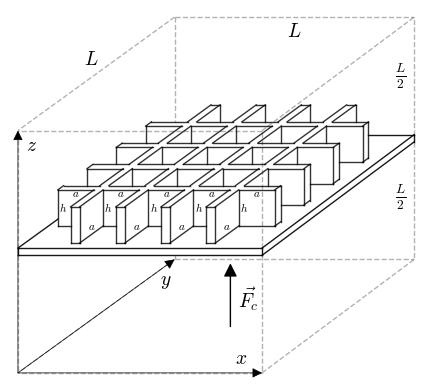
\includegraphics[width=0.42\textwidth]{honeycomb_box_L.png}
\caption{}{\centering{\textbf{Рис.2.} Кубический резонатор с пластиной, покрытой сотами.}}
\end{center}
\label{fig:honeycomb_box_L}
\end{figure}

Результирующая
сила равна
\end{multicols}
\[
F_z = \oint_{\partial V_{\mathrm{vac}}} \langle T_{zz}\rangle \, da
= \big[\langle T_{zz}\rangle_{z=+L/2} - \langle T_{zz}\rangle_{z=-L/2}\big]\,S .
\]
\begin{multicols}{2}




\vspace{\myvspacebeforesubsection}
\subsection*{\centering{\fontencoding{T2A}\fontfamily{ptm}{\selectfont Где стандартный вывод неполон.}}}
\vspace{\myvspaceaftersubsection}

Переход от объёмных сил к натяжениям опирается на теорему Гаусса, которую Тамм
применяет (\S\,33, ф.~33.7) при явном условии \emph{непрерывности} компонент
тензора натяжений внутри объёма; поверхности разрыва там исключены, а позже
(\S\,34, ф.~34.8) рассматриваются лишь их поверхностные \emph{заряды}. Граница
вакуум--металл резонатора может не нести поверхностного заряда и всё же давать
конечный скачок тензора натяжений: тензор, вычисленный по полям со стороны вакуума,
отличается от тензора, вычисленного по полям внутри стенки. Тогда на противоположные
стороны такого элемента поверхности действуют \emph{не} равные и не противоположные
натяжения. Этот случай не рассмотрен ни в \S\,33, ни где-либо в книге Тамма,
включая \S\,105. Для объёма $V$, содержащего внутренние поверхности разрыва $S_j$,
теорему Гаусса нужно записывать в виде
\end{multicols}
\[
\int_V \frac{\partial T_{ik}}{\partial x_k}\,dV
= \oint_{\partial V_{\mathrm{ext}}} T_{ik}\,n_k\,dS
\;-\; \sum_j \int_{S_j} [\![\,T_{ik}\,]\!]\,n_k\,dS_j ,
\]
\begin{multicols}{2}

Поскольку грани лежат в вакууме, это поток импульса \emph{поля} через
чисто вакуумную границу, а не сила, приложенная непосредственно к веществу
пластины. Разность отлична от нуля лишь потому, что структура мод —
а значит, и $\langle T_{zz}\rangle$ — различна на сотовой и на
гладкой стороне. Именно этот член теряется, когда баланс сводится
к $\mathbf{g}=\mathbf{S}/c^2$ при $\langle\mathbf{S}\rangle=0$.

Количественно поверхностный интеграл воспроизводит тягу, полученную ранее из
разности удельных плотностей энергии \cite{Drozdov2024}: для золотых
наносот с размером ячейки $a\approx 2~$мкм
\[
\frac{F}{S} = \langle T_{zz}\rangle_{\mathrm{honey}} - \langle T_{zz}\rangle_{\mathrm{smooth}}
\approx 8{,}55~\text{дин/м}^2 = 8{,}55\times10^{-5}~\text{Н/м}^2 ,
\]
что имеет порядок $\langle T_{zz}\rangle \sim K\,\hbar c/a^4$ с безразмерным
геометрическим коэффициентом $K\sim 4\times10^{-2}$, определяемым структурой мод ячейки.
Таким образом, прочтение через \S\,105 не выводит силу заново, а \emph{интерпретирует} её:
то же самое число есть поток импульса поля через вакуумную границу.

где $[\![\cdot]\!]$ --- скачок величины при переходе через $S_j$. Привычное
отождествление импульса поля с $\mathbf{g}=\mathbf{S}/c^2$ сохраняет лишь внешний
поверхностный интеграл и теряет скачковые члены.

\textbf{Скачок на сотовой пластине.}

У пластины две такие внутренние границы: дно ячеек на структурированной стороне и
гладкая грань на другой. Натяжение на каждой из них --- это электромагнитное давление
вакуумных мод. В приложении~B работы \cite{Drozdov2024} это давление на грань $xy$
прямоугольного резонатора $a\times b\times h$, $f_z/S=\int(H_x^2+H_y^2)\,dS/(8\pi S)$,
вычислено помодово и сопоставлено с плотностью энергии моды $E/V$. Для волны,
распространяющейся вдоль $z$,
\end{multicols}
\[
\frac{f_z/S}{E/V}=1 \quad\text{(электрическая мода, } H_z=0\text{)},
\qquad
\frac{f_z/S}{E/V}=\frac{a^2k_z^2}{a^2k_z^2+\pi^2(n_x^2+n_y^2)} \quad\text{(магнитная мода, } E_z=0\text{)},
\]
\begin{multicols}{2}
и для мод любого типа $\lim_{k_z\to\infty}(f_z/S)/(E/V)=1$. После суммирования по
модам нулевых колебаний скачок $\langle T_{zz}\rangle$ на каждой границе
определяется, таким образом, плотностью энергии вакуума прилегающей полости, а
разность двух скачков даёт
\[
\frac{F}{S}=[\![\langle T_{zz}\rangle]\!]_{\mathrm{honey}}-[\![\langle T_{zz}\rangle]\!]_{\mathrm{smooth}}
\;\ge\;\delta\frac{E}{V}=\hbar c\,\pi\frac{R}{a^4},
\]
то есть неравенство из \cite{Drozdov2024} (приложение~B). Оно совпадает с
гамильтоновым результатом $\partial\langle H\rangle/\partial l$ предыдущего раздела.
Для золотых наносот с ячейкой $a\approx 2~$мкм это даёт
$F/S\approx 8{,}55~\text{дин/м}^2 = 8{,}55\times10^{-5}~\text{Н/м}^2$.
Таким образом, прочтение \S\,105, дополненное скачковыми членами, не выводит силу
заново, а \emph{указывает её место}: несбалансированный импульс находится в скачке
вакуумного тензора натяжений на внутренних границах, который теряется при сведении
к $\mathbf{g}=\mathbf{S}/c^2$.

\textbf{Эквивалентная форма через «коробочку».}
Если охватить всю пластину поверхностью-«коробочкой» $\partial V_{\mathrm{vac}}$ с
гранями в свободном вакууме при $z=\pm d$ (боковые грани сокращаются в силу симметрии
в плоскости), сумма скачков превращается во внешний поток,
$F_z=\oint_{\partial V_{\mathrm{vac}}}\langle T_{zz}\rangle\,da
=\big[\langle T_{zz}\rangle_{z=+d}-\langle T_{zz}\rangle_{z=-d}\big]S$.
Это поток импульса \emph{поля} через чисто вакуумную границу; он отличен от нуля лишь
потому, что структура мод, а значит и $\langle T_{zz}\rangle$, различна на сотовой и
на гладкой стороне.

Два замечания делают интерпретацию однозначной.
Во-первых, не сохраняется импульс именно \emph{поля} (или, что то же, материальной
пластины, которая его поглощает), а не полный импульс замкнутой лабораторной системы;
полный импульс пластины, поля и опоры сохраняется --- точно так же, как у обычного
паруса на ветру. Во-вторых, перенормированное вакуумное натяжение
$\langle T_{\mu\nu}\rangle$ является физически измеряемой величиной --- это и есть
сам эффект Казимира, --- поэтому скачковые члены не требуют предположения о
материальном эфире: их значение задаётся тем же $\langle T_{\mu\nu}\rangle$, которое
подтверждено экспериментально для симметричной конфигурации. Именно нарушенная
трансляционная симметрия граничных условий, а не самого пространства, делает
$\partial\langle H\rangle/\partial l\neq 0$.



\vspace{\myvspacebeforesubsection}
\subsection*{\centering{\fontencoding{T2A}\fontfamily{ptm}{\selectfont ЗАКЛЮЧЕНИЕ}}}
\vspace{\myvspaceaftersubsection}

Сотовый двигатель Казимира является примером физической системы, в которой теорема Нётер непосредственно
объясняет происхождение макроскопической силы: \textbf{отсутствие пространственной однородности приводит
к несохранению импульса}, а следовательно, к появлению тяги. Это показывает, что квантовые
вакуумные эффекты — не просто математические артефакты, а проявления глубоких принципов симметрии.
Экспериментальная проверка может не только подтвердить реальность виртуальных фотонов, но и
подтвердить связь между геометрией, симметрией и динамикой в квантовой теории поля.

\end{multicols}

\newpage

\fontencoding{T2A}\fontfamily{ptm}\selectfont

\section*{\centering {\fontencoding{T2A}\fontfamily{ptm}{\selectfont \uppercase{\MyTitleUkr}}}}

\centerline{\Large{\mynameukr \,\orcidlink{\myorcidlink} }}
\vspace{3mm}
\centerline{\textit{\myworkplaceukr}}
\centerline{\textit{E-mail: \href{mailto:\myemail}{\myemail}}}

\vspace{3mm}
\centerline{\myreceivedukr}
\centerline{\myacceptedukr}

\vspace{3.5mm}

У цій роботі аналізується стільниковий рушій Казимира через призму теореми Нетер.
Розглянута система — ідеально провідна пластина з нанорозмірною стільниковою структурою
з одного боку — не має трансляційної симетрії вздовж осі, нормальної до пластини,
через геометричну асиметрію вакуумних мод з двох її сторін. Як наслідок,
гамільтоніан вакууму явно залежить від координати \(l\) (ефективної довжини резонатора),
і, згідно з теоремою Нетер, відповідна компонента імпульсу не зберігається.
Це незбереження проявляється як результуюча сила квантового вакууму (тяга Казимира).
Показано, що отриманий вираз для сили на одиницю площі безпосередньо відображає цю порушену
симетрію й узгоджується як з гамільтоновим підходом, так і з різницею густин енергії.
Результат підкреслює глибокий фізичний принцип: макроскопічна тяга від квантових флуктуацій
вакууму виникає саме тому, що система не є інваріантною відносно просторових зсувів.
Окремо показано, що стандартне застосування рівняння балансу імпульсу (\S\,105 Тамма)
є неповним для систем із $\langle\mathbf{S}\rangle=0$: оскільки середній вектор Пойнтінга
дорівнює нулю, незбалансований імпульс міститься у поверхневому інтегралі тензора натягів
Максвелла по межі вакуумної області, а не у потоці $\mathbf{g}=\mathbf{S}/c^2$. Не
зберігається імпульс \emph{поля} (речовини), а не повний імпульс замкненої системи;
величина сили спирається на виміряний вакуумний тензор $\langle T_{\mu\nu}\rangle$ і не
потребує припущення про матеріальний ефір.

\begin{thebibliography}{9}
\bibitem{Drozdov2024}
А. Дроздов, \textit{Сотовый двигатель Казимира: о силе, действующей на идеально проводящие соты на пластине}, Вестник Харьковского национального университета имени В.~Н.~Каразина, серия «Физика», вып. 41, 28--41 (2024). \url{https://doi.org/10.26565/2222-5617-2024-41-04}
\bibitem{Noether1918}
E. Noether, \textit{Invariante Variationsprobleme}, Nachr. d. König. Gesellsch. d. Wiss. zu Göttingen, Math-phys. Klasse, 235–257 (1918).
\bibitem{Casimir1948}
H. B. G. Casimir, \textit{On the attraction between two perfectly conducting plates}, Proc. K. Ned. Akad. Wet. B \textbf{51}, 793 (1948).
\bibitem{Tamm1957}
И. Е. Тамм, \textit{Основы теории электричества} (\S\,105, тензор натяжений Максвелла и баланс импульса электромагнитного поля), Наука, Москва.
\bibitem{Feynman1939}
R. P. Feynman, \textit{Forces in molecules}, Phys. Rev. \textbf{56}, 340 (1939).
\bibitem{BrownMaclay1969}
L. S. Brown, G. J. Maclay, \textit{Vacuum stress between conducting plates: an image solution}, Phys. Rev. \textbf{184}, 1272 (1969).
\bibitem{Weyl1912}
H. Weyl, \textit{Das asymptotische Verteilungsgesetz der Eigenwerte linearer partieller Differentialgleichungen}, Math. Ann. \textbf{71}, 441 (1912).
\bibitem{DLP1961}
И. Е. Дзялошинский, Е. М. Лифшиц, Л. П. Питаевский, \textit{Общая теория ван-дер-ваальсовых сил}, УФН \textbf{73}, 381 (1961).
\end{thebibliography}

\end{document}
